\documentclass[dvipsnames, hidelinks]{beamer}

% Enables the use of colour.
\usepackage{xcolor}
% Syntax high-lighting for code. Requires Python's pygments.
\usepackage{minted}
% Enables the use of umlauts and other accents.
\usepackage[utf8]{inputenc}
% Diagrams.
\usepackage{tikz}
% Settings for captions, such as sideways captions.
\usepackage{caption}
% Symbols for units, like degrees and ohms.
\usepackage{gensymb}
% Latin modern fonts - better looking than the defaults.
\usepackage{lmodern}
% Allows for columns spanning multiple rows in tables.
\usepackage{multirow}
% Better looking tables, including nicer borders.
\usepackage{booktabs}
% More math symbols.
\usepackage{amssymb}
% More math layouts, equation arrays, etc.
\usepackage{amsmath}
% More math fonts, like mathbb.
\usepackage{amsfonts}
% More theorem environments.
\usepackage{amsthm}
% More column formats for tables.
\usepackage{array}
% Adjust the sizes of box environments.
\usepackage{adjustbox}
% Better looking single quotes in verbatim and minted environments.
\usepackage{upquote}
% Better blank space decisions.
\usepackage{xspace}
% Better looking tikz trees.
\usepackage{forest}
% URLs.
\usepackage{hyperref}
% For plotting.
\usepackage{pgfplots}

% Various tikz libraries.
% For drawing mind maps.
\usetikzlibrary{mindmap}
% For adding shadows.
\usetikzlibrary{shadows}
% Extra arrows tips.
\usetikzlibrary{arrows.meta}
% Old arrows.
\usetikzlibrary{arrows}
% Automata.
\usetikzlibrary{automata}
% For more positioning options.
\usetikzlibrary{positioning}
% Creating chains of nodes on a line.
\usetikzlibrary{chains}
% Fitting node to contain set of coordinates.
\usetikzlibrary{fit}
% Extra shapes for drawing.
\usetikzlibrary{shapes}
% For markings on paths.
\usetikzlibrary{decorations.markings}
% For advanced calculations.
\usetikzlibrary{calc}

% GMIT colours.
\definecolor{gmitblue}{RGB}{20,134,225}
\definecolor{gmitred}{RGB}{220,20,60}
\definecolor{gmitgrey}{RGB}{67,67,67}

% Change some style options.
\usetheme{metropolis}
\usemintedstyle{manni}
\setbeamercolor{structure}{fg=gmitblue}
\setbeamercolor{frametitle}{fg=white, bg=gmitred}
\setbeamercolor{alerted text}{fg=gmitblue}
\usefonttheme[onlymath]{serif}

% \citeurl can be used to a clickable short url to a slide as a reference.
\renewcommand\footnoterule{}
\newcommand{\citeurl}[1]{\let\thefootnote\relax\footnotetext{\tiny \textcolor{gmitgrey}{\href{http://#1}{#1}}}}
\newcommand{\citeeg}[1]{\let\thefootnote\relax\footnotetext{\tiny \textcolor{gmitgrey}{#1}}}

% A basic horizontal rule.
\newcommand{\hr}{\rule{\textwidth}{0.5pt}}

% Prevent minted from showing errors.
\makeatletter
\expandafter\def\csname PYGdefault@tok@err\endcsname{\def\PYGdefault@bc##1{{\strut ##1}}}
\makeatother

\begin{document}
  \title{Thompson's construction}
  \subtitle{}
  \author{ian.mcloughlin@gmit.ie}
  \date{}

  \begin{frame}
    \titlepage
  \end{frame}

  \begin{frame}[fragile]{Thompson's construction}
  \begin{description}
    \item[Algorithm] to construct an Non-deterministic Finite Automaton (NFA) from a regular expression.
    \item[NFA] will recognise the same language as the regular expression.
  \end{description}
  \vspace{6mm}
  \begin{alertblock}{Example: $a.b|b^*$}
    \vspace{2mm}
    \begin{adjustbox}{max width={0.8\textwidth}, center} 
      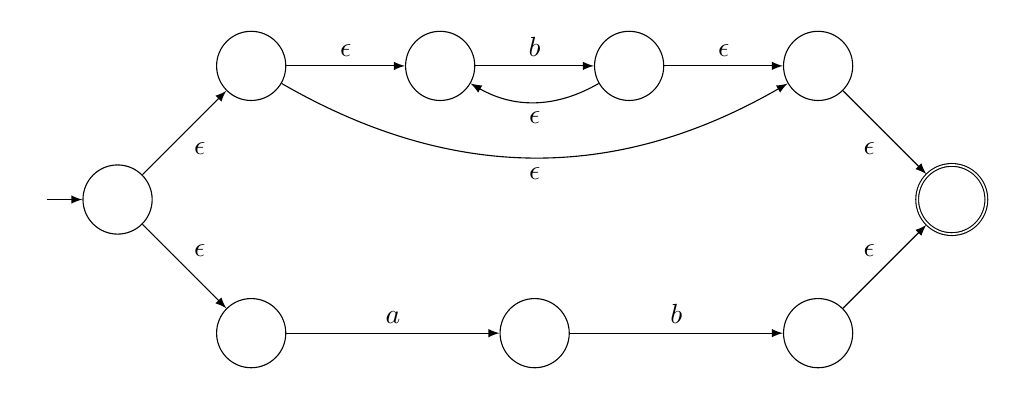
\begin{tikzpicture}[auto, on grid, node distance=24mm, initial text=, >=latex]

        \node[state, initial]            (q_1)                      {}; 
        \node[state]                     (q_2) [above right of=q_1] {};
        \node[state]                     (q_3) [below right of=q_1] {};

        \node[state]                     (q_4) [      right of=q_2] {};
        \node[state]                     (q_5) [      right of=q_4] {};
        \node[state]                     (q_6) [      right of=q_5] {};
        
        \node[state, node distance=36mm] (q_7) [      right of=q_3] {};
        \node[state, node distance=36mm] (q_8) [      right of=q_7] {};

        \node[state, accepting]          (q_9) [below right of=q_6] {}; 


        \path[->]
          (q_1) edge [below right]       node {$\epsilon$} (q_2)
                edge []                  node {$\epsilon$} (q_3)

          (q_2) edge []                  node {$\epsilon$} (q_4)
                edge [bend right, below] node {$\epsilon$} (q_6)
          (q_4) edge []                  node {$b$}        (q_5)
          (q_5) edge []                  node {$\epsilon$} (q_6)
                edge [bend left, below]  node {$\epsilon$} (q_4)
          (q_6) edge [below left]        node {$\epsilon$} (q_9)

          (q_3) edge []                  node {$a$}        (q_7)
          (q_7) edge []                  node {$b$}        (q_8)
          (q_8) edge []                  node {$\epsilon$} (q_9);

      \end{tikzpicture}
    \end{adjustbox}
  \end{alertblock}
\end{frame}


\begin{frame}[fragile]{Fragments}
  \begin{description}
    \item[Assume] the regular expression is in postfix.
    \item[Stack] of fragments of the overall NFA.
    \item[Normal] characters push to the stack.
    \item[Special] characters pop from and push to the stack.
  \end{description}
  \vspace{6mm}
  \begin{alertblock}{Example fragment}
    \vspace{2mm}
    \begin{adjustbox}{max width={0.8\textwidth}, center} 
      \begin{tikzpicture}[auto, on grid, node distance=24mm, initial text=, >=latex]

        \node[state, initial, fill=gmitblue]  (q_1) [] {};
        \node[state]                          (q_2) [right of=q_1] {};
        \node[state]                          (q_3) [right of=q_2] {};
        \node[state, accepting, fill=gmitred] (q_4) [right of=q_3] {};


        \path[->]
          (q_1) edge []                  node {$\epsilon$} (q_2)
                edge [bend right, below] node {$\epsilon$} (q_4)
          (q_2) edge []                  node {$b$}        (q_3)
          (q_3) edge []                  node {$\epsilon$} (q_4)
                edge [bend left, below]  node {$\epsilon$} (q_2);

        \begin{scope}[on background layer]
          \node[cloud, draw=black, fill=gmitgrey!20, cloud puffs=30, cloud puff arc=110, aspect=5, minimum width=68mm, minimum height=36mm] at (3.6,-0.3) {};
        \end{scope}
      \end{tikzpicture}
    \end{adjustbox}
  \end{alertblock}
\end{frame}


\begin{frame}[fragile]{Non-special characters}
  For a normal, non-special character $x$ push the following fragment to the stack.
  
  \vspace{4mm}
  
  \begin{adjustbox}{max width={0.8\textwidth}, center} 
    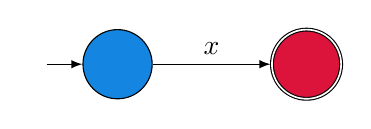
\begin{tikzpicture}[auto, on grid, node distance=24mm, initial text=, >=latex]
      \node[state, initial, fill=gmitblue]  (q_1) [] {};
      \node[state, accepting, fill=gmitred] (q_2) [right of=q_1] {};

      \path[->] (q_1) edge [] node {$x$} (q_2);
    \end{tikzpicture}
  \end{adjustbox}

  \vspace{4mm}

  We should include the empty regular expression $\epsilon$ too.
  
  \vspace{10mm}

  \begin{adjustbox}{max width={0.8\textwidth}, center} 
    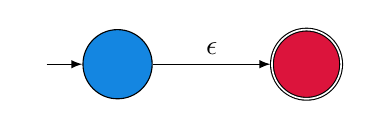
\begin{tikzpicture}[auto, on grid, node distance=24mm, initial text=, >=latex]
      \node[state, initial, fill=gmitblue]  (q_1) [] {};
      \node[state, accepting, fill=gmitred] (q_2) [right of=q_1] {};

      \path[->] (q_1) edge [] node {$\epsilon$} (q_2);
    \end{tikzpicture}
  \end{adjustbox}
\end{frame}


\begin{frame}[fragile]{Concatenation $N.M$}
  When you see a $.$, pop two fragments from the stack and push the following instead.
  
  \vspace{18mm}
  
  \begin{adjustbox}{max width={\textwidth}, center}
    \begin{tikzpicture}[auto, on grid, node distance=24mm, initial text=, >=latex]
      
      \node[state, initial, fill=gmitblue]   (a_1)   []               {};
      \node[draw=none,fill=none]             (namea) [right of=a_1]   {Fragment 2};
      \node[state, fill=gmitred!50!gmitblue] (a_2)   [right of=namea] {};

      \node[draw=none,fill=none]             (nameb) [right of=a_2]   {Fragment 1};
      \node[state, fill=gmitred, accepting]  (b_2)   [right of=nameb] {};

      \begin{scope}[on background layer]
        \node[cloud, draw=black, fill=gmitgrey!20, cloud puffs=30, cloud puff arc=110, aspect=5, minimum width=50mm, minimum height=20mm, right of=a_1] {};
        \node[cloud, draw=black, fill=gmitgrey!20, cloud puffs=30, cloud puff arc=110, aspect=5, minimum width=50mm, minimum height=20mm, right of=a_2] {};
      \end{scope}
    \end{tikzpicture}
  \end{adjustbox}
\end{frame}


\begin{frame}[fragile]{Union $N|M$}
  When you see a $|$, pop two fragments from the stack and push the following instead.
  
  \vspace{4mm}
  
  \begin{adjustbox}{max width={0.8\textwidth}, center}
    \begin{tikzpicture}[auto, on grid, node distance=24mm, initial text=, >=latex]
      \node[state, initial, fill=gmitblue]  (s_i)   []                   {};
      
      \node[state, fill=gmitblue!50]        (a_1)   [above right of=s_i] {};
      \node[draw=none,fill=none]            (namea) [right of=a_1]       {Fragment 1};
      \node[state, fill=gmitred!50]         (a_2)   [right of=namea]     {};

      \node[state, fill=gmitblue!50]        (b_1)   [below right of=s_i] {};
      \node[draw=none,fill=none]            (nameb) [right of=b_1]       {Fragment 2};
      \node[state, fill=gmitred!50]         (b_2)   [right of=nameb]     {};

      \node[state, accepting, fill=gmitred] (s_a)   [below right of=a_2] {};

      \path[->] (s_i) edge [below right] node {$\epsilon$} (a_1)
                      edge [above right] node {$\epsilon$} (b_1)
                (a_2) edge [below left]  node {$\epsilon$} (s_a)
                (b_2) edge []            node {$\epsilon$} (s_a);
              

      \begin{scope}[on background layer]
        \node[cloud, draw=black, fill=gmitgrey!20, cloud puffs=30, cloud puff arc=110, aspect=5, minimum width=50mm, minimum height=20mm, right of=b_1] {};
        \node[cloud, draw=black, fill=gmitgrey!20, cloud puffs=30, cloud puff arc=110, aspect=5, minimum width=50mm, minimum height=20mm, right of=a_1] {};
      \end{scope}
    \end{tikzpicture}
  \end{adjustbox}
\end{frame}

\begin{frame}[fragile]{Kleene star $N^*$}
  When you see a $^*$, pop a fragment from the stack and push the following instead.
  
  \vspace{10mm}
  
  \begin{adjustbox}{max width={0.8\textwidth}, center}
    \begin{tikzpicture}[auto, on grid, node distance=24mm, initial text=, >=latex]
      \node[state, initial, fill=gmitblue]  (s_i)   []               {};
      
      \node[state, fill=gmitblue!50]        (a_1)   [right of=s_i]   {};
      \node[draw=none,fill=none]            (namea) [right of=a_1]   {Fragment};
      \node[state, fill=gmitred!50]         (a_2)   [right of=namea] {};

      \node[state, accepting, fill=gmitred] (s_a)   [right of=a_2]   {};

      \path[->] (s_i) edge []                     node {$\epsilon$} (a_1)
                      edge [bend right=40, below] node {$\epsilon$} (s_a)
                (a_2) edge []                     node {$\epsilon$} (s_a)
                      edge [bend right=90, above] node {$\epsilon$} (a_1);
              

      \begin{scope}[on background layer]
        \node[cloud, draw=black, fill=gmitgrey!20, cloud puffs=30, cloud puff arc=110, aspect=5, minimum width=50mm, minimum height=20mm, right of=a_1] {};
      \end{scope}
    \end{tikzpicture}
  \end{adjustbox}
\end{frame}


\begin{frame}{Data structures}
  Recall the definition of an NFA.
  \begin{description}
    \item[$Q$] is a finite set of \emph{states},
    \item[$\Sigma$] is a finite set called the \emph{alphabet},
    \item[$\delta$] is the \emph{transition function} ($Q \times \Sigma_{\epsilon} \rightarrow \mathcal{P}(Q)$),
    \item[$q_0$] is the \emph{start state} ($\in Q$), and
    \item[$F$] is the set of \emph{accept states} ($\subseteq Q$). 
  \end{description}

  \begin{alertblock}{Notes}
    \begin{itemize}
      \item Only need to know $\delta$, $q_0$ and $F$, and $|F| = 1$.
      \item Nothing points at $q_0$ and $q_f$ points at nothing.
      \item From every state is a single symbol arrow or two $\epsilon$ arrows.
    \end{itemize}
  \end{alertblock}
\end{frame} 
\end{document}
 